\section{Results}
\label{sec:results}

18400 windows were extracted from the data, which resulted in more than 36000 strides. A total of 11,900 windows were labeled, with 7,450 and 4,450 labeled as "ridden" during walk and trot, respectively, while the remaining 3,550 and 2,950 were labeled as "not-ridden" during walk and trot. 

The best and the worst performing models were based on random forest and \gls{svm}, respectively. The performance results of the random forest models per gait were presented in detail in Table \ref{tab:rider_results}, and were compared with other algorithms in Table \ref{tab:rider_compared} (models trained based on sacrum+limb \gls{imu}s and walk+trot gait). For visual comparison, the accuracy results of the random forest models per gait are demonstrated in Figure \ref{fig:rider_three} and compared with other machine learning models in Figure \ref{fig:rider_four}. Furthermore, the accuracy, sensitivity, and specificity of the models resulting from testing on walk+trot data are depicted in Figure \ref{fig:rider_five}. 

\begin{table}[!htbp] 
\centering
\caption{Performance of random forest models per gait}% Add 'table' caption
\resizebox{0.75\linewidth}{!}{%
\begin{tabular}{llccc}
\toprule
\textbf{\gls{imu}} & 
\textbf{Gait type} & \textbf{Accuracy}& \textbf{Sensitivity}& \textbf{Specificity}\\
\midrule 
    
Sacrum + Limb & Walk + Trot & 97.4\% & 97.2\% & 97.9\%\\
              & Walk & 96.6\% & 95.3\% & 99.4\%\\
              & Trot & 98.6\% & 99.9\% & 95.6\%\\
\midrule
Sacrum & Walk + Trot & 87.6\% & 87.3\% & 88.4\%\\
       & Walk & 86.4\% & 84.0\% & 91.4\%\\
       & Trot & 89.5\% & 92.1\% & 83.7\%\\
\midrule
Limb & Walk + Trot & 92.9\% & 97.8\% & 82.4\%\\
     & Walk & 92.1\% & 97.1\% & 81.4\%\\
     & Trot & 94.2\% & 98.8\% & 83.9\%\\

        \bottomrule         
    \label{tab:rider_results}
  \end{tabular}
  }

\end{table}
\begin{table}[!htbp] 
\centering
\caption{Performance of the models with different input features trained on Sacrum+Limb data during Walk+Trot}% Add 'table' caption
\resizebox{0.65\linewidth}{!}{%
\begin{tabular}{llccc}
\toprule
\textbf{Model} & 
\textbf{Features} & \textbf{Accuracy}& \textbf{Sensitivity}& \textbf{Specificity}\\
\midrule 
    
Random forest & All     & 97.4\% & 97.2\% & 97.9\%\\
          & Top ten & 90.9\% & 87.3\% & 98.8\%\\
\midrule
Decision tree  & All     & 94.4\% & 93.2\% & 97.0\%\\
          & Top ten & 84.3\% & 88.8\% & 74.5\%\\
\midrule
\gls{lda} & All     & 91.9\% & 88.9\% & 98.4\%\\
          & Top ten & 88.7\% & 99.2\% & 65.8\%\\
\midrule
\gls{svm} & All     & 90.6\% & 92.4\% & 86.7\%\\
          & Top ten & 87.4\% & 99.3\% & 61.5\%\\

        \bottomrule         
    \label{tab:rider_compared}
  \end{tabular}
  }

\end{table}

\begin{figure}[htbp]
\centering
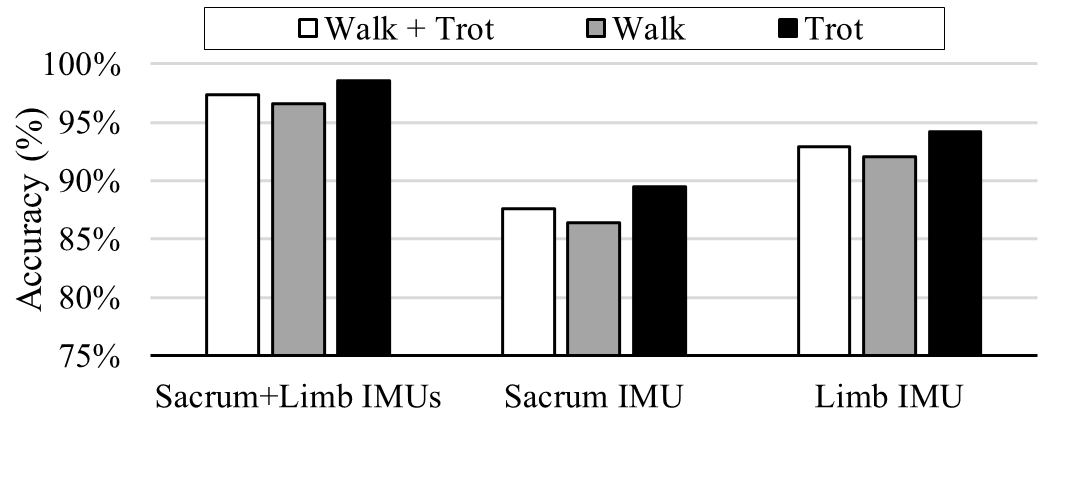
\includegraphics[width=.8\linewidth]{chapters/rider/figures/Picture3.png}
\caption{Accuracy of the random forest models per gait}
\label{fig:rider_three}
\end{figure}

\begin{figure}[htbp]
\centering
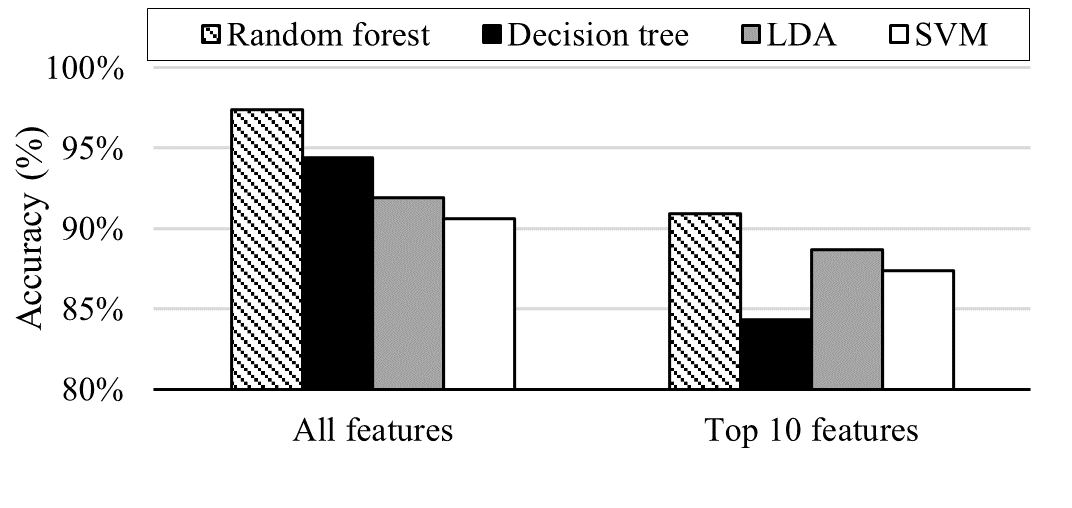
\includegraphics[width=.8\linewidth]{chapters/rider/figures/Picture4.png}
\caption{Accuracy of the models with different number of input features trained on Sacrum+Limb data during Walk+Trot}
\label{fig:rider_four}
\end{figure}

\begin{figure}[htbp]
\centering
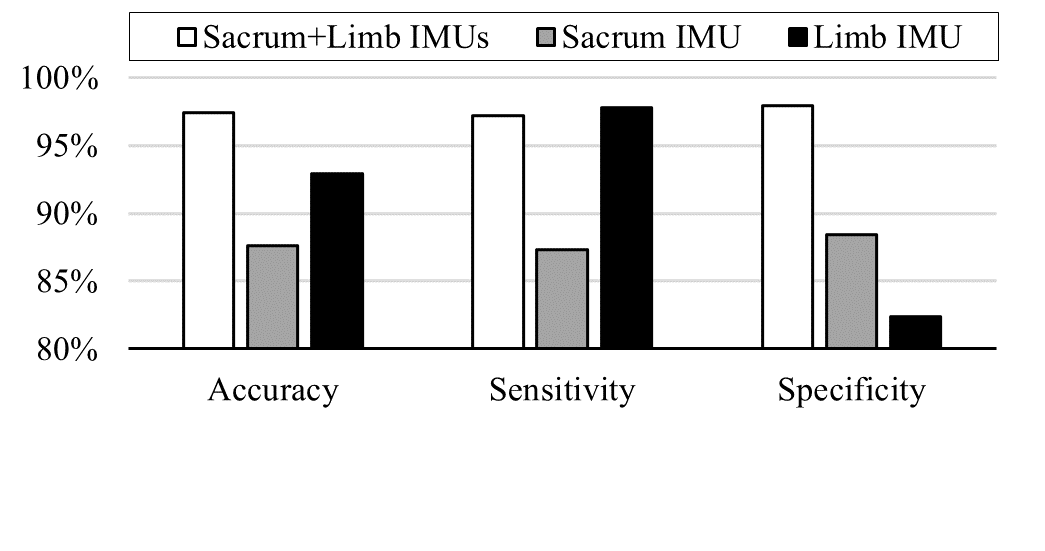
\includegraphics[width=.8\linewidth]{chapters/rider/figures/Picture5.png}
\caption{Accuracy, sensitivity, and specificity of the models based on random forest using Walk+Trot data}
\label{fig:rider_five}
\end{figure}

It can be inferred from Table \ref{tab:rider_results} that the model based on Sacrum+Limb \gls{imu}s features yielded the best performance during walk, trot, and Walk+Trot. Between the two other models based on one \gls{imu}, the model based on limb \gls{imu} features performed better than the model based on sacrum \gls{imu} except for the specificity of walking data. Moreover, the performance of the models when using trotting data was slightly higher than walking data.

\begin{table}[!htbp] 
\centering
\caption{The ten highest ranked features from \gls{nca}}% Add 'table' caption
\resizebox{\linewidth}{!}{%
\begin{tabular}{lllll}
\toprule
\textbf{Rank} & 
\textbf{Feature description} & \textbf{\gls{imu}}& \textbf{Signal}& \textbf{Axis}\\
\midrule 
    
1  & Magnitude of \gls{fft} first coefficient & Sacrum      & Acceleration                  & Along vertical (z-axis)\\
2  & Angular range of motion                  & Limb        & Angle                         & Around longitudinal (x-axis)\\
3  & Maximum value                            & Limb        & Angular velocity              & Around protraction angle (z-axis)\\
4  & Angular range of motion                  & Limb        & Angle                         & Around protraction angle (z-axis)\\
5  & Angular range of motion                  & Limb        & Angle                         & Around adduction angle (y-axis)\\
6  & Standard deviation                       & Sacrum      & Angular velocity              & Around longitudinal (x-axis)\\
7  & Median value                             & Sacrum      & Acceleration                  & Along longitudinal (z-axis)\\
8  & Linear range of motion                   & Sacrum      & Displacement                  & Along vertical (z-axis)\\
9  & Swing duration                           & Limb/ & Acceleration/ & -\\[-5pt]
   &                                          & Sacrum   & Angular velocity              &  \\
10 & Linear range of motion                   & Limb        & Displacement                  & Along longitudinal (x-axis)\\
        \bottomrule         
    \label{tab:rider_features_results}
  \end{tabular}
  }

\end{table}

Using the weights from the output of \gls{nca}, the top ten features were selected and reported in Table \ref{tab:rider_features_results}. In addition, normalized values of the top three features between the two classes were demonstrated in Figure \ref{fig:rider_six}. For model performance comparison based on the number of features, we reported the performance of the models based on the top ten features in Table \ref{tab:rider_features_results}, where five and four features were extracted from limb and sacrum \gls{imu}s, respectively. Out of all the parameters, only one was kinematic, the ninth feature, which represented swing duration. Half of the selected features were directly extracted from the \gls{imu}s raw signals (acceleration and angular velocity). The remaining were calculated from the integration of the raw signals (angle and displacement). 

\begin{figure}[htbp]
\centering
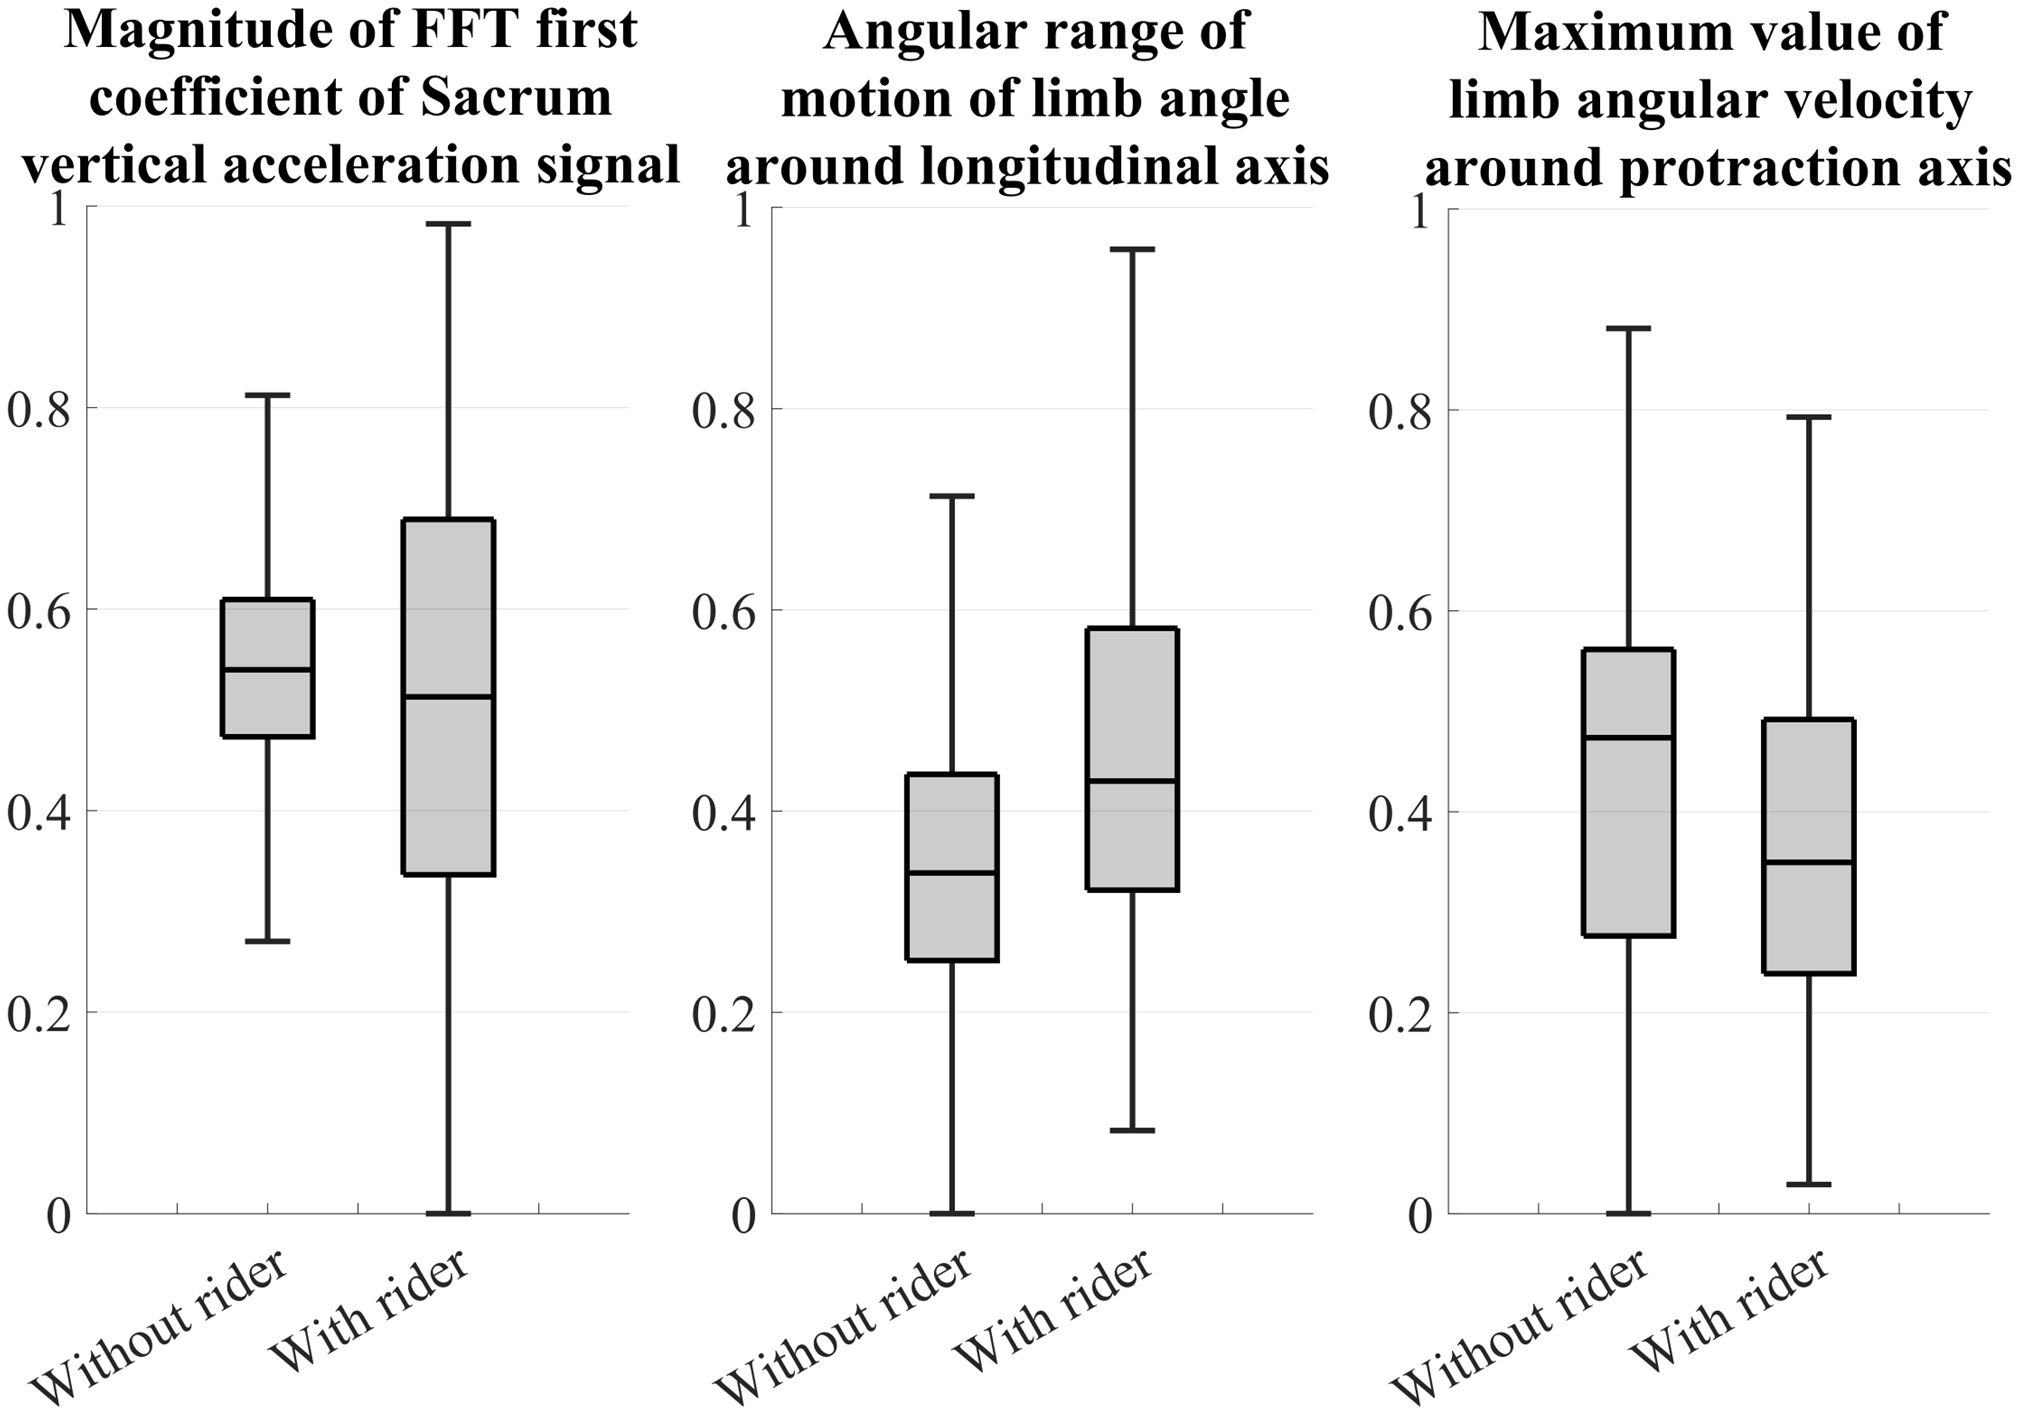
\includegraphics[width=.75\linewidth]{chapters/rider/figures/Picture6.png}
\caption{Normalized values (0 to 1) of the top three features (according to \gls{nca}) between the two classes: without rider and with rider}
\label{fig:rider_six}
\end{figure}
